\documentclass[11pt,a4paper]{article}

% ---- packages ----------------------------------------------------------------
\usepackage[utf8]{inputenc}
\usepackage[T1]{fontenc}
\usepackage[margin=2.4cm]{geometry}
\usepackage{graphicx}
\usepackage{xcolor}
\usepackage{booktabs}
\usepackage{tabularx}
\usepackage{float}
\usepackage{enumitem}
\usepackage{caption}
\usepackage{listings}
\usepackage{fancyhdr}
\usepackage[hidelinks]{hyperref}

% ---- colours -----------------------------------------------------------------
\definecolor{accent}{HTML}{2B4C7E}
\definecolor{muted}{HTML}{66788A}
\definecolor{codebg}{HTML}{F5F7FA}
\definecolor{kw}{HTML}{2B4C7E}
\definecolor{str}{HTML}{1B7F4B}
\definecolor{cmt}{HTML}{8A94A0}

% ---- code listing style ------------------------------------------------------
\lstdefinestyle{py}{
  language=Python,
  backgroundcolor=\color{codebg},
  basicstyle=\ttfamily\footnotesize,
  keywordstyle=\color{kw}\bfseries,
  stringstyle=\color{str},
  commentstyle=\color{cmt}\itshape,
  numberstyle=\tiny\color{muted},
  numbers=left, numbersep=8pt,
  frame=single, rulecolor=\color{muted!40},
  breaklines=true, showstringspaces=false,
  captionpos=b, xleftmargin=14pt, framexleftmargin=14pt,
  tabsize=4,
}

% ---- header / footer ---------------------------------------------------------
\pagestyle{fancy}
\fancyhf{}
\lhead{\small\color{muted}Encrypted Password Manager}
\rhead{\small\color{muted}Digital Security}
\cfoot{\thepage}
\renewcommand{\headrulewidth}{0.3pt}

\captionsetup{font=small,labelfont={bf,color=accent}}
\setlength{\parskip}{0.5em}
\setlength{\parindent}{0pt}

% ---- title -------------------------------------------------------------------
\title{\vspace{-1cm}\color{accent}\textbf{Encrypted Password Manager}\\[0.3cm]
       \large\color{black}Project Documentation --- Digital Security}
\author{Nenu Mihai-Adrian\\ \small Digital Security}
\date{\today}

\begin{document}
\maketitle
\thispagestyle{empty}

\begin{abstract}
\noindent This report documents a local password manager that stores credentials
encrypted and grants access through a single master password. The application
uses AES-256 in GCM mode for authenticated encryption, the memory-hard Scrypt
function for deriving the encryption key from the master password, and an SQLite
database that holds only ciphertext. Both a command-line and a graphical
interface are provided over a shared cryptographic backend. The document
describes the design and its justification, the development steps, the problems
encountered and how they were solved, the automated tests, and an honest
analysis of the threat model and remaining limitations.
\end{abstract}

\tableofcontents
\newpage

% =============================================================================
\section{Overview and relevance}
Passwords are still the primary authentication mechanism online, and the reuse
of weak passwords is one of the most common causes of account compromise. A
password manager solves this by letting the user remember a single strong
secret --- the \emph{master password} --- while every account receives a long,
unique, randomly generated password.

This project implements such a manager as a small, self-contained application
and demonstrates several core topics of digital security in practice:
symmetric encryption (AES-256-GCM), key derivation from a human password
(Scrypt), encryption at rest, integrity and tamper detection through
authenticated encryption, and cryptographically secure random generation.

% =============================================================================
\section{How the requirements are satisfied}
The brief required AES-256, one of Argon2 / scrypt / PBKDF2, and encrypted
SQLite. Table~\ref{tab:req} maps each requirement to its implementation.

\begin{table}[H]
\centering
\renewcommand{\arraystretch}{1.35}
\begin{tabularx}{\textwidth}{@{}p{4.2cm}X@{}}
\toprule
\textbf{Requirement} & \textbf{Implementation} \\
\midrule
AES-256 & AES-256-GCM (\texttt{AESGCM} from the \texttt{cryptography} library), 256-bit key. \\
Argon2 / scrypt / PBKDF2 & \textbf{Scrypt}, a memory-hard KDF, with $N=2^{15}$, $r=8$, $p=1$. \\
Encrypted SQLite & Every credential is AES-GCM encrypted \emph{before} being written; the file holds only opaque blobs and non-secret KDF parameters. \\
Master-password access & The key is derived from the master password at runtime; a stored \emph{verifier} confirms correctness without storing the password. \\
\bottomrule
\end{tabularx}
\caption{Mapping of brief requirements to the implementation.}
\label{tab:req}
\end{table}

\paragraph{Note on Argon2 vs Scrypt.} The brief allows any of the three KDFs.
Argon2id is the modern first choice, but it requires a third-party package that
was unavailable in the build environment. Scrypt is also memory-hard, ships
inside the audited \texttt{cryptography} library, and fully satisfies the
requirement. The code isolates key derivation in a single function, so switching
to Argon2id later is a one-line change.

% =============================================================================
\section{Architecture}
The application is split into three layers so that cryptography, storage and the
user interface remain independent and testable.

\begin{table}[H]
\centering
\renewcommand{\arraystretch}{1.35}
\begin{tabularx}{\textwidth}{@{}p{3.6cm}X@{}}
\toprule
\textbf{File} & \textbf{Responsibility} \\
\midrule
\texttt{crypto\_utils.py} & Scrypt key derivation, AES-256-GCM encrypt/decrypt, secure password generation. No knowledge of storage. \\
\texttt{vault.py} & Opens the SQLite file, verifies the master password, performs encrypted create/read/update/delete. \\
\texttt{pwmanager.py} & Command-line interface. \\
\texttt{pwmanager\_gui.py} & Graphical interface (Tkinter) over the same backend. \\
\texttt{selftest.py} & Automated functional and security tests. \\
\bottomrule
\end{tabularx}
\caption{Project modules and their responsibilities.}
\end{table}

% =============================================================================
\section{Cryptographic design and justification}

\subsection{Deriving the key (Scrypt)}
A human password is far too weak and short to be used directly as an AES key. It
is passed through Scrypt, which stretches it into a 32-byte (256-bit) key, mixes
in a random 16-byte salt so that identical master passwords yield different keys
(defeating precomputed tables), and is memory-hard --- roughly 32~MB per
attempt with the chosen parameters --- making large-scale brute-force guessing
extremely costly while a single legitimate unlock stays fast.

\begin{lstlisting}[style=py,caption={Key derivation with Scrypt.}]
def derive_key(master_password, salt, n=2**15, r=8, p=1):
    kdf = Scrypt(salt=salt, length=32, n=n, r=r, p=p)  # 32 bytes = AES-256
    return kdf.derive(master_password.encode("utf-8"))
\end{lstlisting}

\subsection{Encrypting the data (AES-256-GCM)}
Every secret is encrypted with AES-256 in GCM mode. GCM is preferred over a
plain mode such as CBC because it is \emph{authenticated}: it provides
confidentiality and, through its authentication tag, integrity and
authenticity. Any modification of the ciphertext is detected at decryption time,
which gives tamper detection for free. Two rules are enforced: a fresh random
96-bit nonce is generated for every encryption (nonce reuse in GCM is
catastrophic), and associated data binds each ciphertext to its role.

\begin{lstlisting}[style=py,caption={Authenticated encryption; a unique nonce per call.}]
def encrypt(key, plaintext, associated_data=b""):
    aes = AESGCM(key)
    nonce = secrets.token_bytes(12)          # unique per encryption
    return nonce + aes.encrypt(nonce, plaintext, associated_data)
\end{lstlisting}

\subsection{Verifying the master password}
We must be able to report a wrong password without storing the password or key.
At vault creation a known constant is encrypted with the derived key and saved
as a \emph{verifier}. On unlock, a candidate key is derived and used to decrypt
the verifier: success means the password is correct; an authentication failure
means it is wrong. The verifier leaks nothing --- it is just another ciphertext.

\subsection{What the database contains}
Because the entire entry (title, username, password, URL, notes, timestamps) is
inside the encrypted blob, an attacker who steals the file learns only how many
entries exist. This is the sense in which the SQLite storage is ``encrypted'':
encryption is applied at the application level to every value before it reaches
the database.

% =============================================================================
\section{Installation and running}
Requirements: Python 3.10+ and the \texttt{cryptography} package; the GUI also
uses \texttt{tkinter}, bundled with standard Python / Anaconda.

\begin{lstlisting}[style=py,caption={Running the application.}]
pip install -r requirements.txt
python3 pwmanager_gui.py     # graphical interface
python3 pwmanager.py         # command-line interface
\end{lstlisting}

% =============================================================================
\section{User interface}
The graphical interface presents an unlock screen, an entry list with live
search, and a details panel from which a stored password can be revealed or
copied.

\begin{figure}[H]
\centering
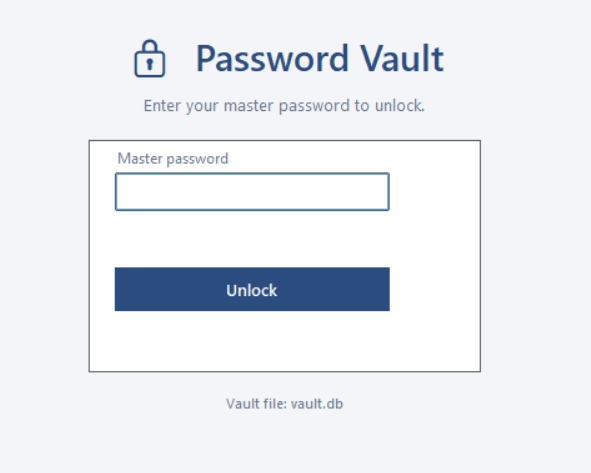
\includegraphics[width=0.55\textwidth]{screenshots/unlock.png}
\caption{Unlock / create screen. The master password is entered hidden.}
\end{figure}

\begin{figure}[H]
\centering
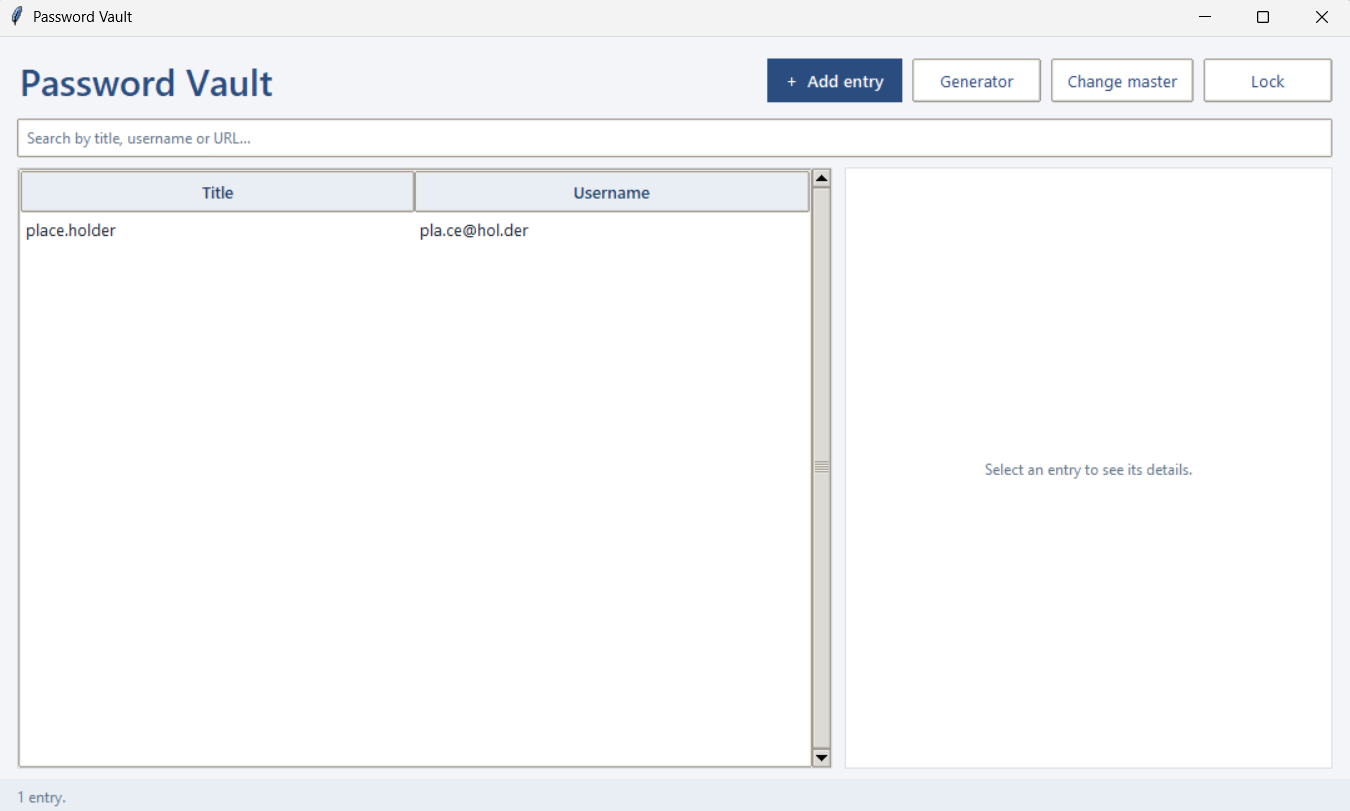
\includegraphics[width=0.9\textwidth]{screenshots/main.png}
\caption{Main window: entry list on the left, details on the right.}
\end{figure}

\begin{figure}[H]
\centering
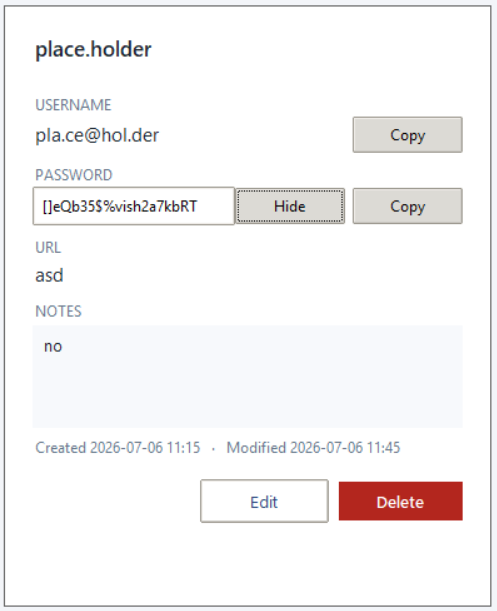
\includegraphics[width=0.9\textwidth]{screenshots/view-password.png}
\caption{Viewing a stored password via the Show/Hide toggle, with one-click copy
and automatic clipboard clearing.}
\end{figure}

\begin{figure}[H]
\centering
\begin{minipage}{0.48\textwidth}
  \centering
  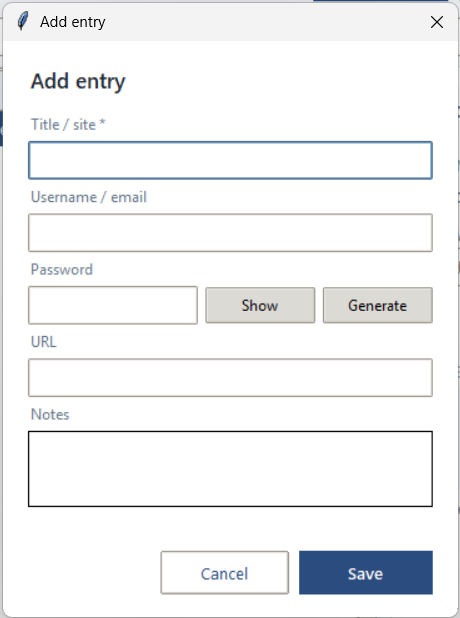
\includegraphics[width=\textwidth]{screenshots/add-entry.png}
  \caption{Add / edit dialog with a built-in generator.}
\end{minipage}\hfill
\begin{minipage}{0.48\textwidth}
  \centering
  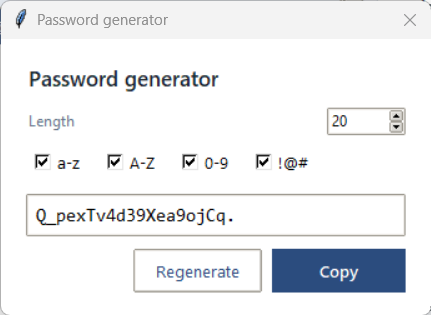
\includegraphics[width=\textwidth]{screenshots/generator.png}\\[0.6cm]
  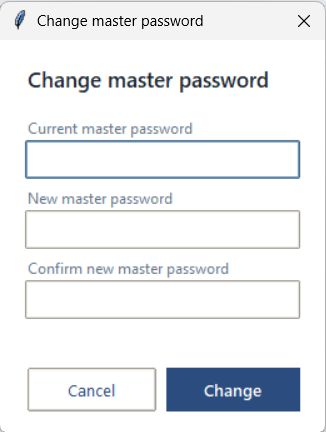
\includegraphics[width=\textwidth]{screenshots/change-master.png}
  \caption{Password generator and master-password change.}
\end{minipage}
\end{figure}

% =============================================================================
\section{Development steps}
\begin{enumerate}[leftmargin=1.4em]
  \item Chose a layered architecture (crypto / storage / UI) so each concern
        could be tested independently.
  \item Implemented \texttt{crypto\_utils.py}: Scrypt derivation, AES-GCM
        helpers, and a CSPRNG-based password generator.
  \item Built \texttt{vault.py}: the two-table schema, initialize/unlock flow,
        the verifier mechanism, and encrypted CRUD.
  \item Added the master-password change routine with full re-encryption inside
        a single transaction.
  \item Wrote the command-line interface, then a polished Tkinter GUI over the
        same backend.
  \item Wrote an automated self-test and iterated until every check passed.
\end{enumerate}

% =============================================================================
\section{Problems encountered and solutions applied}

\begin{table}[H]
\centering
\renewcommand{\arraystretch}{1.4}
\begin{tabularx}{\textwidth}{@{}XX@{}}
\toprule
\textbf{Problem} & \textbf{Solution} \\
\midrule
Argon2 unavailable (no package, no network). & Used Scrypt, memory-hard and part of the \texttt{cryptography} library; the KDF is isolated so Argon2id can replace it with one line. \\
Detecting a wrong master password without storing password or key. & A \emph{verifier}: a known constant encrypted with the key; correct key decrypts it, wrong key fails authentication. \\
``Encrypted SQLite'' without a native full-disk library. & Application-level encryption: every value is AES-GCM encrypted before storage, so the file is only ciphertext. \\
GCM nonce reuse would break security. & A fresh random 96-bit nonce for every encryption, stored with each ciphertext. \\
Ciphertext role confusion (swapping blobs). & Associated data binds each ciphertext to its purpose (entry vs.\ verifier). \\
Atomicity while changing the master password. & Re-encrypt everything inside a single transaction with rollback on error. \\
Metadata leaking through the database. & Store the whole entry inside the encrypted blob, so only the entry count is visible. \\
\bottomrule
\end{tabularx}
\caption{Problems encountered during development and the solutions applied.}
\end{table}

% =============================================================================
\section{Testing}
The script \texttt{selftest.py} runs twelve automated checks, all passing:
initialization and unlock; add and retrieve round-trip; sorted listing; search;
update; delete; a locked vault refusing access; wrong-password rejection and
correct acceptance; \textbf{no plaintext of any secret in the raw database
file}; master-password change re-encrypting all data; \textbf{tamper detection}
when a stored blob is modified; and generator output of the requested length
containing all character classes.

% =============================================================================
\section{Critical analysis, threat model and limitations}
\textbf{Protected against:} theft of the database file (only ciphertext at
rest), offline brute-force of the master password (slowed massively by Scrypt),
and silent modification of stored data (detected by GCM authentication).

\textbf{Not protected against (honest limitations):} a compromised machine while
the vault is unlocked (the key and decrypted secrets live in RAM, and Python
cannot reliably wipe them); a weak master password, which no KDF can rescue; and
metadata such as the number of entries, which remains visible.

\textbf{Possible improvements:} replace Scrypt with Argon2id; adopt SQLCipher for
transparent full-file encryption that also hides metadata; add an auto-lock
timeout (already present in the GUI), a clipboard copy with automatic clearing
(also present), and a breach/reuse checker; and provide encrypted export/import
for backups.

% =============================================================================
\section{Conclusion}
The application meets the brief: it stores credentials encrypted with AES-256-GCM,
derives the key from the master password with the memory-hard Scrypt function,
and persists only ciphertext in SQLite. Beyond the minimum, it adds tamper
detection, a strong password generator, master-password re-keying, auto-lock,
and both a command-line and a graphical interface, together with a documented
threat model that states clearly what the design does and does not protect
against.

\end{document}
